\section{Procesar una Dimensión} 

1. Ya creada la dimensión, el siguiente paso es Procesarla para ver la generación de los datos. En la pestaña
de Dimension Structure ubicamos la opción de Process:

	\begin{center}
	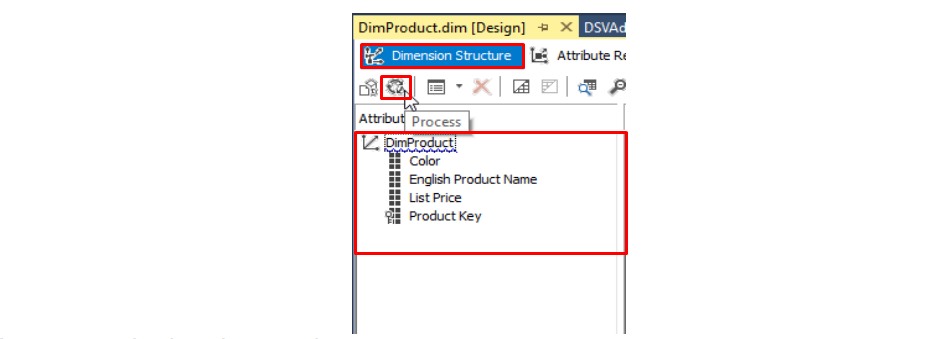
\includegraphics[width=\columnwidth]{images/task2/img13}
	\end{center}	

2. Nos mostrará un mensaje de advertencia:

	\begin{center}
	
\includegraphics[width=\columnwidth]{images/task2/img14}
    \end{center}	
    
Click en Yes.

3. Luego Click en Run…
Se nos abrirá una ventana donde nos mostrará el progreso del proceso de la dimensión DimProduct:
	\begin{center}
	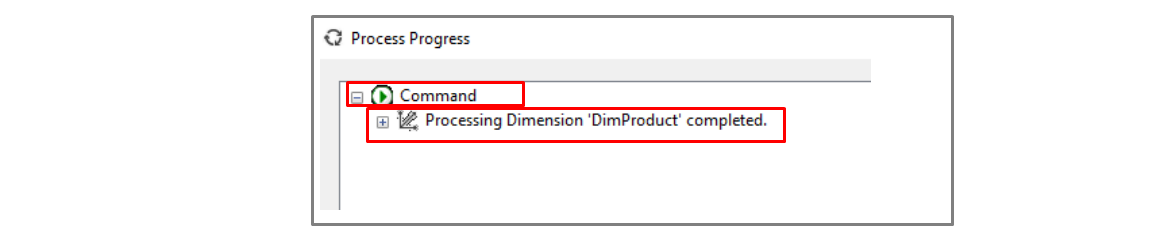
\includegraphics[width=\columnwidth]{images/task2/img17}
    \end{center}	
    

4. En la pestaña de Browser exploramos los atributos y los valores que contienen.
Exploramos el atributo Color:

	\begin{center}
	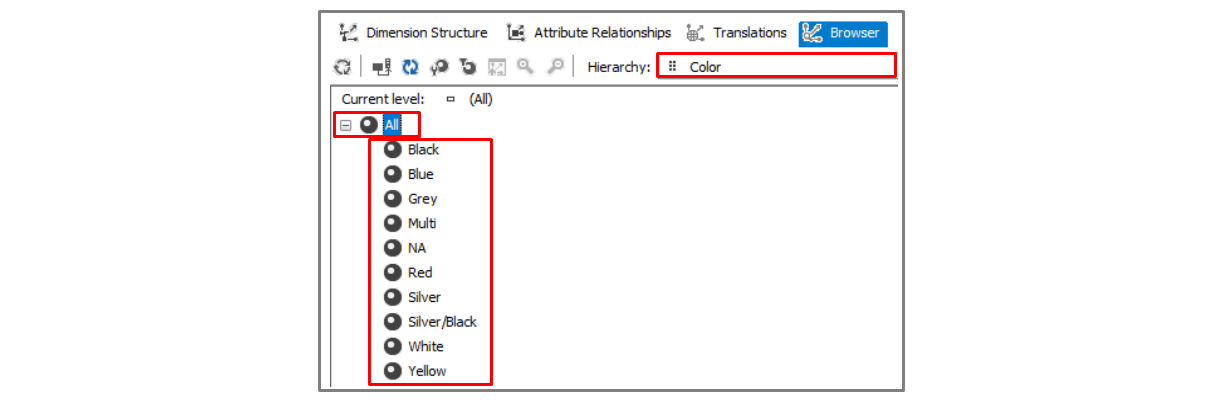
\includegraphics[width=\columnwidth]{images/task2/img19}
    \end{center}	
    
5. Exploramos el atributo English Product Name:
    \begin{center}
	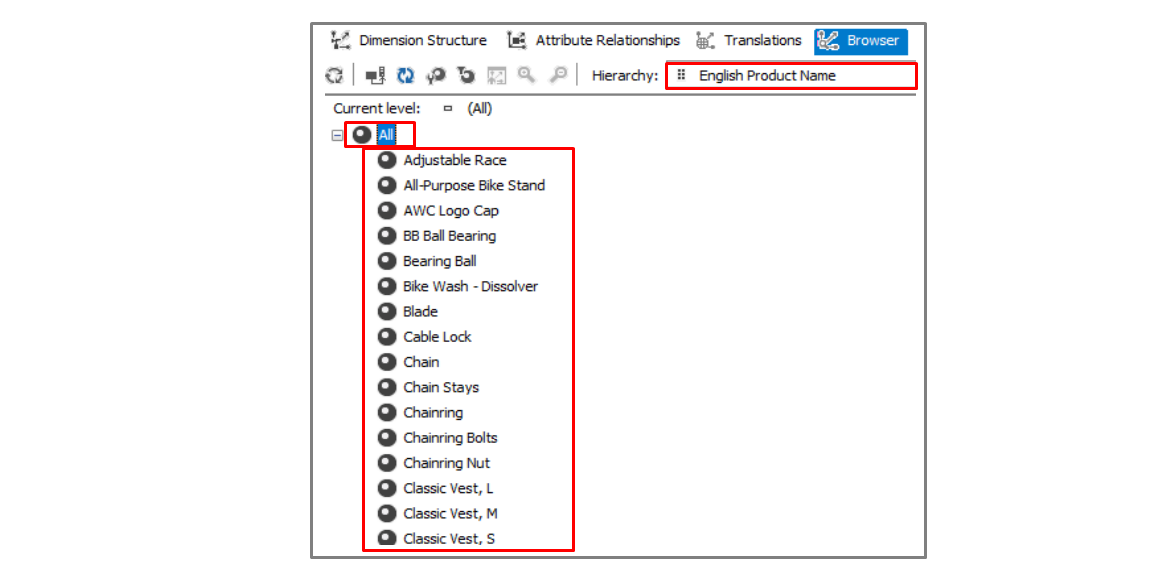
\includegraphics[width=\columnwidth]{images/task2/img21}
    \end{center}	
 
6. Exploramos el atributo Product Key:

	\begin{center}
	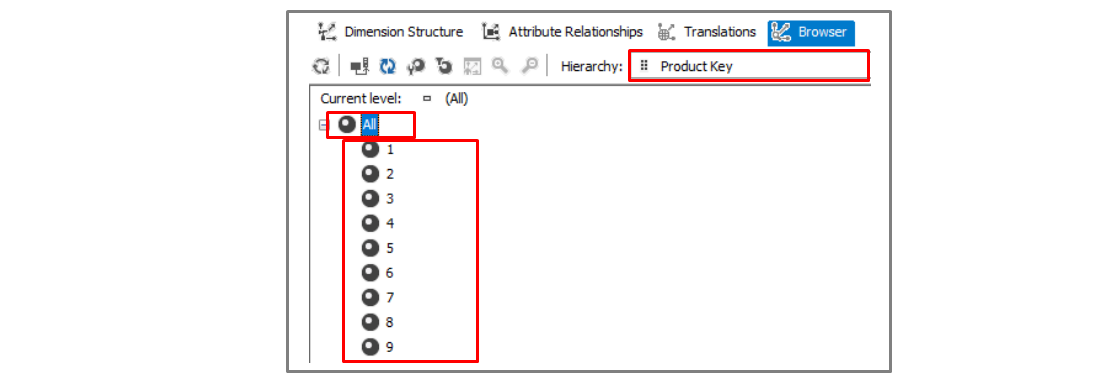
\includegraphics[width=\columnwidth]{images/task2/img22}
    \end{center}	
   
Es aquí donde detectamos que si bien es cierto nos muestra los valores de Product Key , lo recomendable
es que este atributo no sea visible para el usuario final, ya que esta es una llave propia del DW.
	